\documentclass[fontset=windows]{article}
\usepackage[margin=1in]{geometry}
\usepackage{ctex}
\usepackage{setspace}
\usepackage{lipsum}
\usepackage{graphicx}
\usepackage{caption}
\usepackage{subcaption}
\usepackage[colorlinks=true,linkcolor=red]{hyperref}

\graphicspath{{figures/}}

\title{\heiti\zihao{2} Large-Signal \& Small-Signal Operation}
\author{\songti zrrraa}
\date{2023.11.16}

\begin{document}
\maketitle
\thispagestyle{empty}

\section*{MOS in Parallel}

\begin{figure}[htbp]
    \centering
    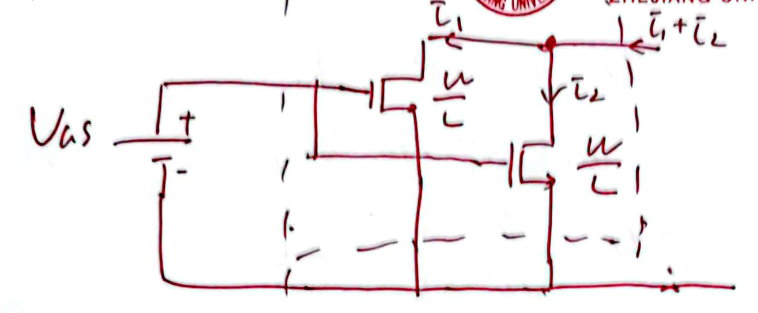
\includegraphics[scale=0.6]{1.jpg}
    \captionsetup{labelformat=empty}
    \caption{}
    \label{1}
\end{figure}

If we place two MOS in parallel as a new MOS, what is the I/V characteristics of new MOS? 

Let's look at it in 3D diagram. 

\begin{figure}[htbp]
    \centering
    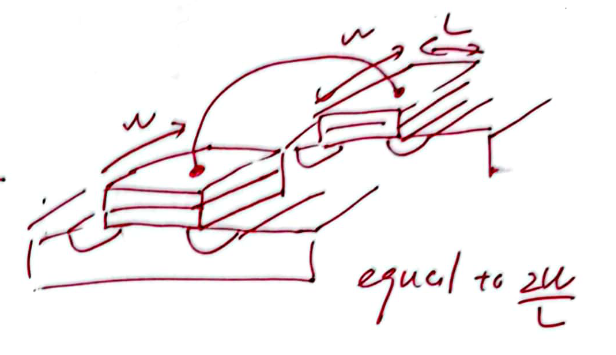
\includegraphics[scale=0.6]{2.jpg}
    \captionsetup{labelformat=empty}
    \caption{}
    \label{2}
\end{figure}

Obviously, the new MOS has a double W/L. Now we derive it in math. 

$$I_1=\frac{1}{2} \mu C_{ox}\frac{W}{L}(V_{GS}-V_{TH})^2$$

$$I_2=\frac{1}{2} \mu C_{ox}\frac{W}{L}(V_{GS}-V_{TH})^2$$

$$I_{new MOS}=I_1+I_2=\frac{1}{2} \mu C_{ox}\frac{2W}{L}(V_{GS}-V_{TH})^2$$

That is, the W/L of the new MOS is twice that of the original. 

$$g_{m1}=\frac{2I_1}{V_{GS}-V_{TH}}$$

$$g_{m2}=\frac{2I_2}{V_{GS}-V_{TH}}$$

$$g_{m}=g_{m1}+g_{m2}=\frac{2I_1+2I_2}{V_{GS}-V_{TH}}=2g_{m1}=2g_{m2}$$

The transconductance of the new MOS is also twice that of the original. 

\section*{Let's build an amplifier}

Last day we didn't take $V_{DS}$ into consideration. In the case we designed yesterday, the MOS didn't work in the saturation zone, 
which means the amplification circuit fails. 

Actually, we also need to add a bias voltage to the Drain. 

\begin{figure}[htbp]
    \centering
    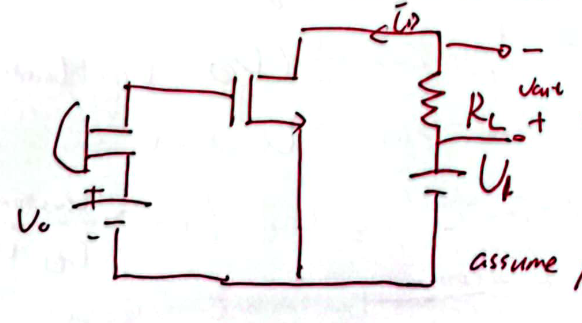
\includegraphics[scale=0.6]{3.jpg}
    \captionsetup{labelformat=empty}
    \caption{Add a bias voltage to the Drain}
    \label{3}
\end{figure}

Assume that $V_D=0.9V$, $V_{TH}=0.5V$, $I_D=1mA$, $R_L=1k\Omega$. 

If $V_{DS}\geq V_0-V_{TH}=0.4V$, the MOS is in saturation zone. 

So if we let $V_1\leq I_{Dmin}*R_L+V_{DS}=1.4V$, the MOS can work in saturation zone. 

In this way, we build an amplifier successfully. 

\section*{Large-Signal Operation}

\begin{figure}[htbp]
    \centering
    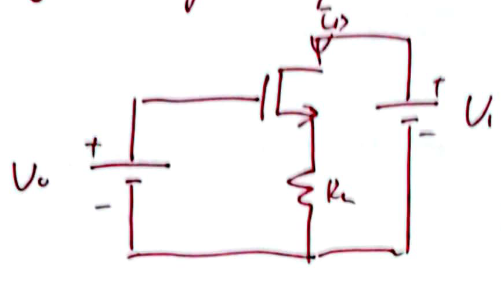
\includegraphics[scale=0.6]{4.jpg}
    \captionsetup{labelformat=empty}
    \caption{Large-Signal Operation}
    \label{4}
\end{figure}

We have: 

$$I_D=\frac{1}{2} \mu C_{ox}\frac{W}{L}(V_{GS}-V_{TH})^2$$

$$V_{GS}=\sqrt{\frac{2I_D}{\mu_nC_ox\frac{W}{L}}}+V_{TH}$$

Then we can get: 

$$V_0=V_{GS}+I_D*R_L=\sqrt{\frac{2I_D}{\mu_nC_{ox}\frac{W}{L}}}+V_{TH}+I_DR_L$$

\subsection*{Let's add a signal}

\begin{figure}[htbp]
    \centering
    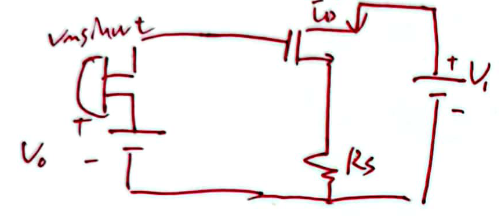
\includegraphics[scale=0.6]{5.jpg}
    \captionsetup{labelformat=empty}
    \caption{Large-Signal Operation}
    \label{5}
\end{figure}

We assume that $V_m$ is not "small". 

$$V_0+V_m sin\omega t=V_{GS}+I_D*R_S=\sqrt{\frac{2I_D}{\mu_nC_{ox}\frac{W}{L}}}+V_{TH}+I_DR_S$$

\section*{Small-Signal Operation}

\begin{figure}[htbp]
    \centering
    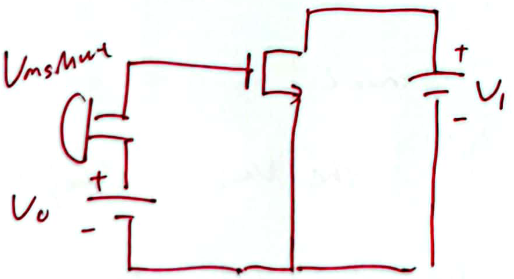
\includegraphics[scale=0.6]{6.jpg}
    \captionsetup{labelformat=empty}
    \caption{Small-Signal Operation}
    \label{6}
\end{figure}

Now we assume that $V_m$ is small, $V_{GS}$ is almost a constant. 

In this case, $I_D$ is almost a constant, we can ignore the $R_s$ too. 

$$I_D=\frac{1}{2} \mu C_{ox}\frac{W}{L}(V_0-V_{TH}+V_{m}sin\omega t)^2$$

Because $V_{GS}-V_{TH}\geq V_msin\omega t$, we have $(1+x)^2\approx 1+2x$. 

Then: 

$$I_D=\frac{1}{2} \mu C_{ox}\frac{W}{L}(V_{0}-V_{TH})^2(1+2\frac{V_msin\omega t}{V_0-V_{TH}})$$

$$I_D=I_{D0}+\frac{2I_{D0}}{V_0-V_{TH}}V_m sin\omega t$$

We call the former Bias Current, and the latter Signal Current. Obviously the Signal Current is $g_m*V_msin\omega t$.  
This fits well with the definition of transconductance, the ability to convert voltage into current. 

$$g_m=\frac{dI_D}{dV_{GS}}$$

$dV_{GS}$ there is the small $V_msin\omega t$.  

According to this, we can also split this circuit into two parts. 

\begin{figure}[htbp]
    \centering
    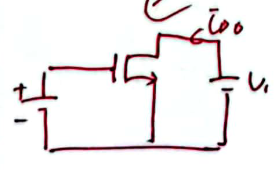
\includegraphics[scale=0.6]{7.jpg}
    \captionsetup{labelformat=empty}
    \caption{Bias Current}
    \label{7}
\end{figure}

\begin{figure}[htbp]
    \centering
    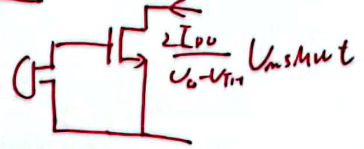
\includegraphics[scale=0.6]{8.jpg}
    \captionsetup{labelformat=empty}
    \caption{Signal Current}
    \label{8}
\end{figure}

Let's take its simple model. 

\begin{figure}[htbp]
    \centering
    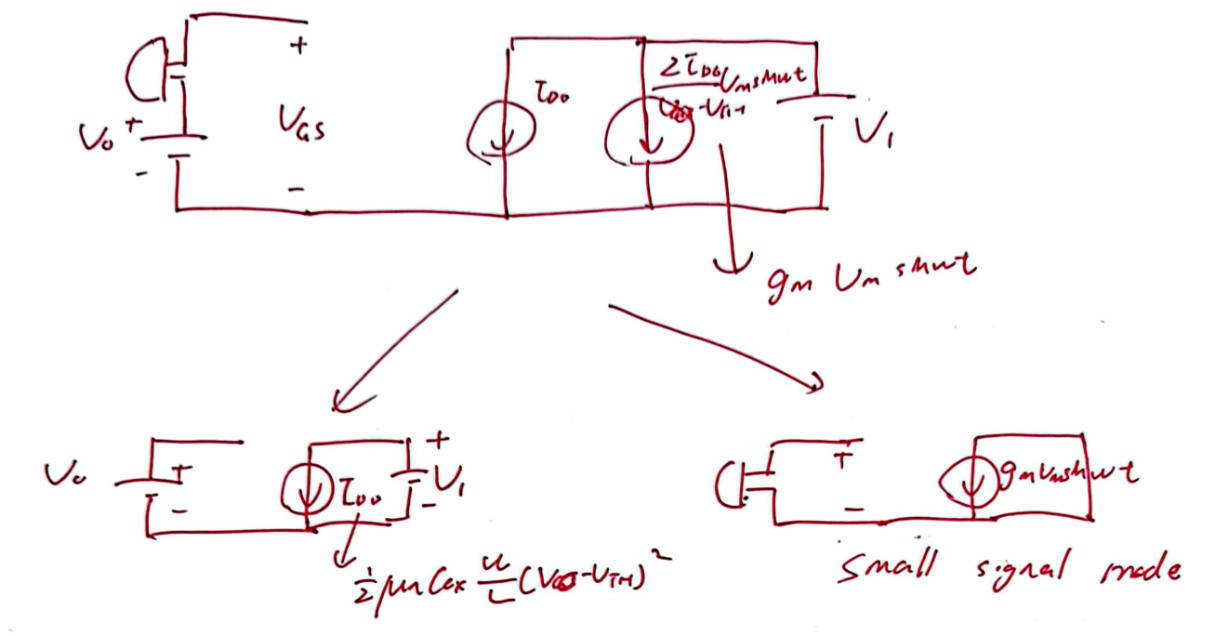
\includegraphics[scale=0.6]{9.jpg}
    \captionsetup{labelformat=empty}
    \caption{}
    \label{9}
\end{figure}

In this way, we split a model into Large-Signal Model and Small-Signal Model. 

Additionally, we can find the Large-Signal Model only has DC component and Small-Signal Model only has AC component. 

\section*{Link}

\href{https://www.bilibili.com/video/BV1FD4y1R7Ah?p=33&vd_source=1d0c07486a3bd3b0adb8ac548bf6453e}{Razavi Electronics Circuits 1: lectrue 33}
\end{document}